\documentclass{standalone}
\usepackage{tikz}
\usetikzlibrary{patterns, positioning}
\usepackage[sfdefault]{ClearSans} %% option 'sfdefault' activates Clear Sans as the default text font
\usepackage[T1]{fontenc}

\begin{document}
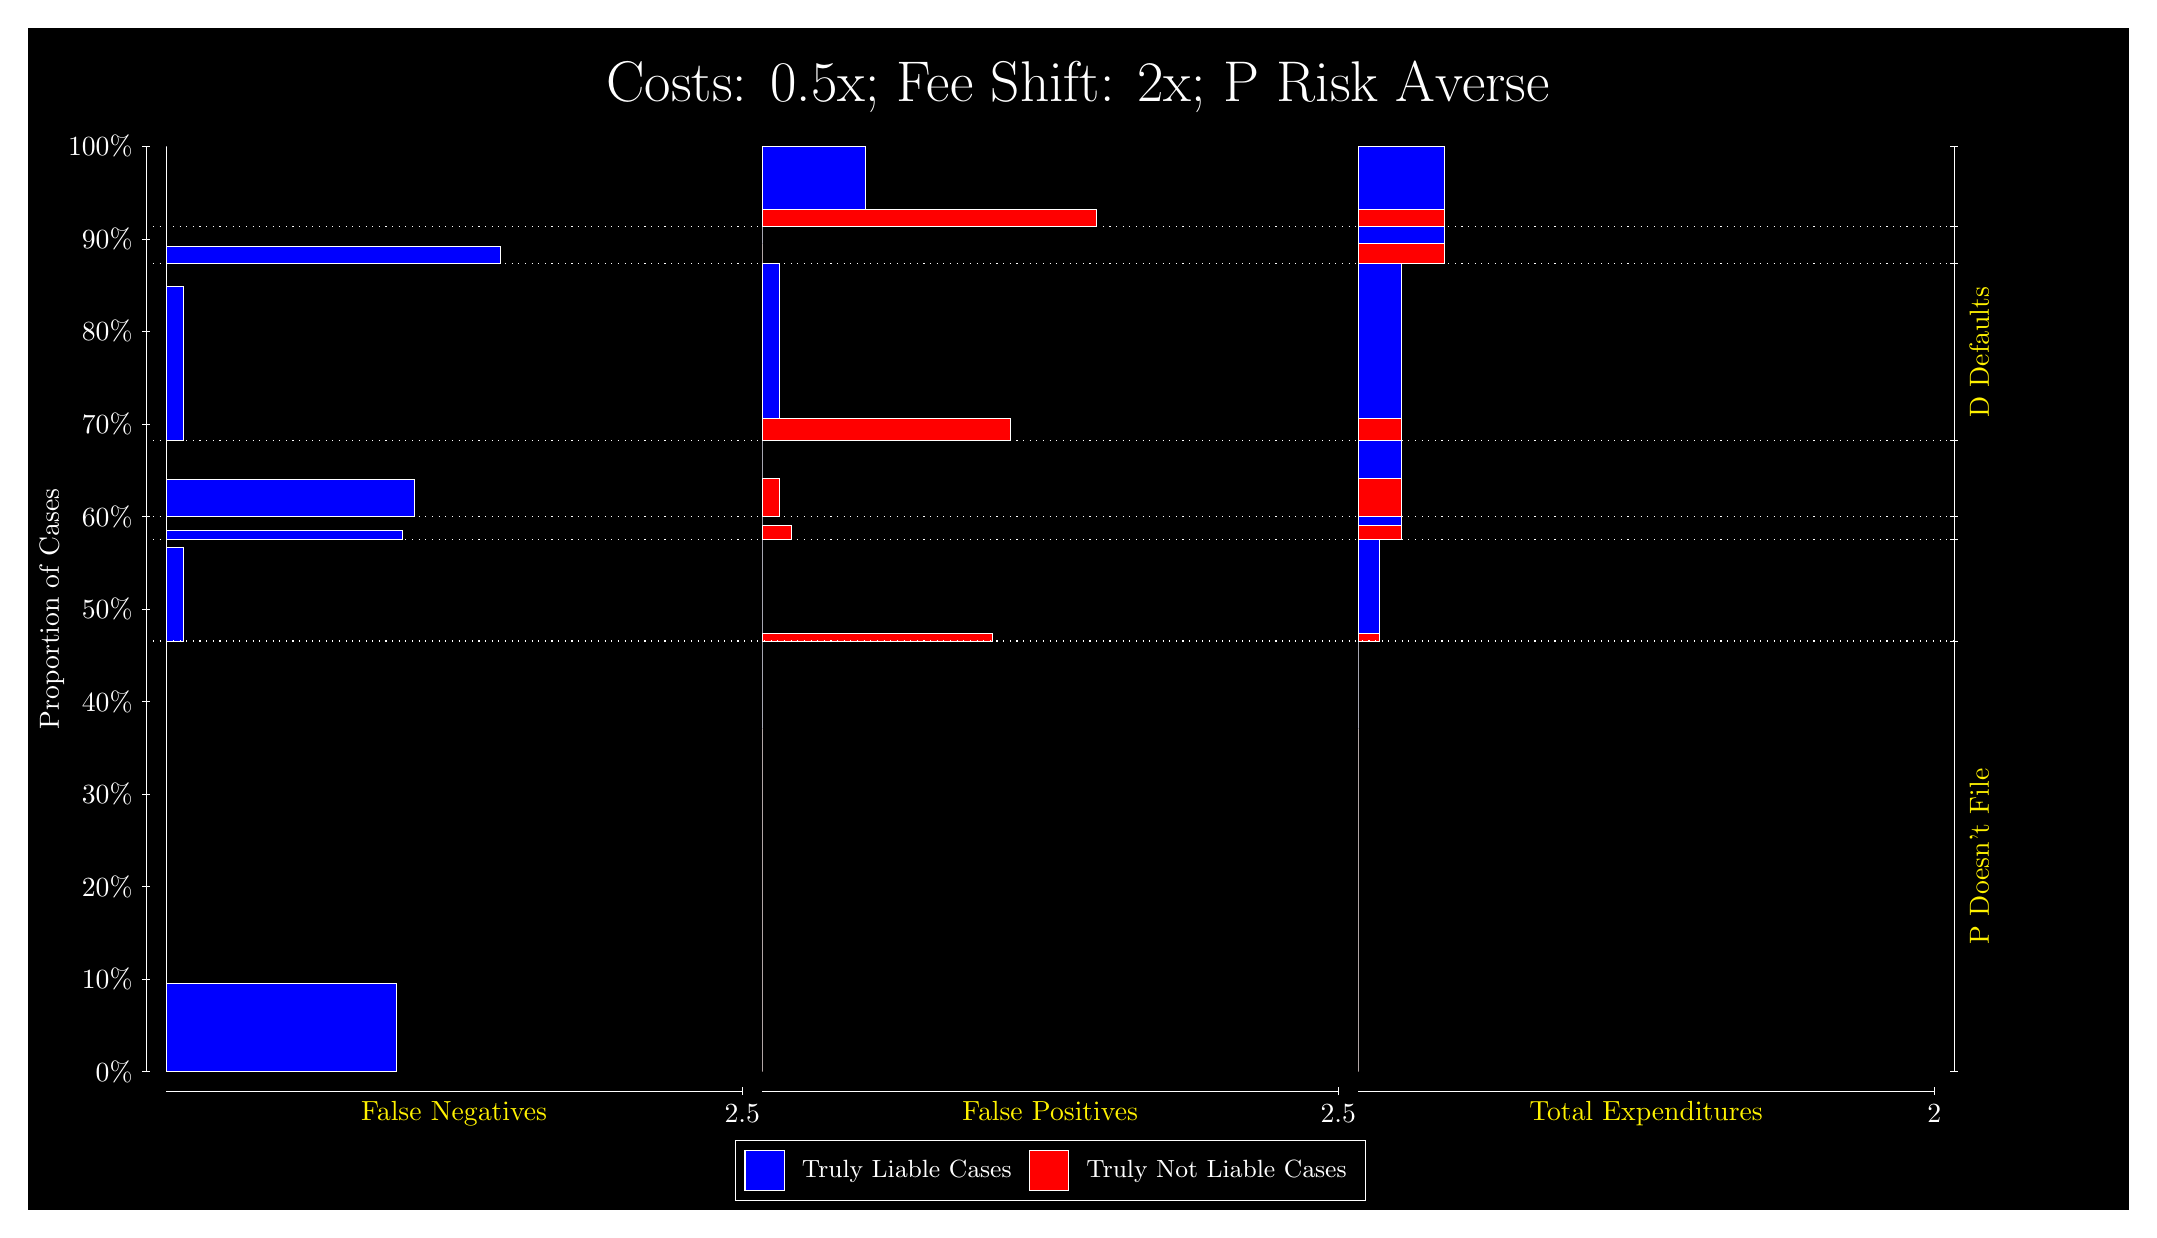
\begin{tikzpicture}
\draw[fill=black] (0,0) rectangle (26.667,15);
\draw[text=white] (0,13.5) rectangle (26.667,15) node[midway] {\huge Costs: 0.5x; Fee Shift: 2x; P Risk Averse};
\draw[white, very thin] (1.5,1.75) -- (1.5,13.5);
\node[rotate=90, text=white, anchor=center] at (0.3, 7.625) {Proportion of Cases};
\draw[white, very thin] (1.45,1.75) -- (1.55,1.75);
\node[text=white, anchor=east] at (1.45, 1.75) {0\%};
\draw[white, very thin] (1.45,2.925) -- (1.55,2.925);
\node[text=white, anchor=east] at (1.45, 2.925) {10\%};
\draw[white, very thin] (1.45,4.1) -- (1.55,4.1);
\node[text=white, anchor=east] at (1.45, 4.1) {20\%};
\draw[white, very thin] (1.45,5.275) -- (1.55,5.275);
\node[text=white, anchor=east] at (1.45, 5.275) {30\%};
\draw[white, very thin] (1.45,6.45) -- (1.55,6.45);
\node[text=white, anchor=east] at (1.45, 6.45) {40\%};
\draw[white, very thin] (1.45,7.625) -- (1.55,7.625);
\node[text=white, anchor=east] at (1.45, 7.625) {50\%};
\draw[white, very thin] (1.45,8.8) -- (1.55,8.8);
\node[text=white, anchor=east] at (1.45, 8.8) {60\%};
\draw[white, very thin] (1.45,9.975) -- (1.55,9.975);
\node[text=white, anchor=east] at (1.45, 9.975) {70\%};
\draw[white, very thin] (1.45,11.15) -- (1.55,11.15);
\node[text=white, anchor=east] at (1.45, 11.15) {80\%};
\draw[white, very thin] (1.45,12.325) -- (1.55,12.325);
\node[text=white, anchor=east] at (1.45, 12.325) {90\%};
\draw[white, very thin] (1.45,13.5) -- (1.55,13.5);
\node[text=white, anchor=east] at (1.45, 13.5) {100\%};

\draw[white, very thin] (24.457,1.75) -- (24.457,13.5);
\draw[white, very thin] (24.407,1.75) -- (24.507,1.75);
\node[anchor=west] at (24.407, 1.75) {};
\draw[white, very thin] (24.407,7.2183) -- (24.507,7.2183);
\node[anchor=west] at (24.407, 7.2183) {};
\draw[white, very thin] (24.407,8.5066) -- (24.507,8.5066);
\node[anchor=west] at (24.407, 8.5066) {};
\draw[white, very thin] (24.407,8.7982) -- (24.507,8.7982);
\node[anchor=west] at (24.407, 8.7982) {};
\draw[white, very thin] (24.407,9.7605) -- (24.507,9.7605);
\node[anchor=west] at (24.407, 9.7605) {};
\draw[white, very thin] (24.407,12.014) -- (24.507,12.014);
\node[anchor=west] at (24.407, 12.014) {};
\draw[white, very thin] (24.407,12.486) -- (24.507,12.486);
\node[anchor=west] at (24.407, 12.486) {};
\draw[white, very thin] (24.407,13.5) -- (24.507,13.5);
\node[anchor=west] at (24.407, 13.5) {};

\draw[white, very thin, fill=blue] (1.75,1.75) rectangle (4.6775,2.8648);
\draw[white, very thin, fill=red] (1.75,2.8648) rectangle (1.75,7.2183);
\draw[white, very thin, fill=blue] (1.75,7.2183) rectangle (1.9696,8.4064);
\draw[white, very thin, fill=red] (1.75,8.4064) rectangle (1.75,8.5066);
\draw[white, very thin, fill=blue] (1.75,8.5066) rectangle (4.7507,8.6222);
\draw[white, very thin, fill=red] (1.75,8.6222) rectangle (1.75,8.7982);
\draw[white, very thin, fill=blue] (1.75,8.7982) rectangle (4.8971,9.2716);
\draw[white, very thin, fill=red] (1.75,9.2716) rectangle (1.75,9.7605);
\draw[white, very thin, fill=blue] (1.75,9.7605) rectangle (1.9696,11.728);
\draw[white, very thin, fill=red] (1.75,11.728) rectangle (1.75,12.014);
\draw[white, very thin, fill=blue] (1.75,12.014) rectangle (5.9949,12.235);
\draw[white, very thin, fill=red] (1.75,12.235) rectangle (1.75,12.486);
\draw[white, very thin, fill=red] (1.75,12.486) rectangle (1.75,12.706);
\draw[white, very thin, fill=blue] (1.75,12.706) rectangle (1.75,13.5);
\draw[white, very thin, fill=red] (9.3189,1.75) rectangle (9.3189,6.1035);
\draw[white, very thin, fill=blue] (9.3189,6.1035) rectangle (9.3189,7.2183);
\draw[white, very thin, fill=red] (9.3189,7.2183) rectangle (12.246,7.3184);
\draw[white, very thin, fill=blue] (9.3189,7.3184) rectangle (9.3189,8.5066);
\draw[white, very thin, fill=red] (9.3189,8.5066) rectangle (9.6848,8.6826);
\draw[white, very thin, fill=blue] (9.3189,8.6826) rectangle (9.3189,8.7982);
\draw[white, very thin, fill=red] (9.3189,8.7982) rectangle (9.5384,9.2871);
\draw[white, very thin, fill=blue] (9.3189,9.2871) rectangle (9.3189,9.7605);
\draw[white, very thin, fill=red] (9.3189,9.7605) rectangle (12.466,10.046);
\draw[white, very thin, fill=blue] (9.3189,10.046) rectangle (9.5384,12.014);
\draw[white, very thin, fill=red] (9.3189,12.014) rectangle (9.3189,12.264);
\draw[white, very thin, fill=blue] (9.3189,12.264) rectangle (9.3189,12.486);
\draw[white, very thin, fill=red] (9.3189,12.486) rectangle (13.564,12.706);
\draw[white, very thin, fill=blue] (9.3189,12.706) rectangle (10.636,13.5);
\draw[white, very thin, fill=red] (16.888,1.75) rectangle (16.888,6.1035);
\draw[white, very thin, fill=blue] (16.888,6.1035) rectangle (16.888,7.2183);
\draw[white, very thin, fill=red] (16.888,7.2183) rectangle (17.162,7.3184);
\draw[white, very thin, fill=blue] (16.888,7.3184) rectangle (17.162,8.5066);
\draw[white, very thin, fill=red] (16.888,8.5066) rectangle (17.437,8.6826);
\draw[white, very thin, fill=blue] (16.888,8.6826) rectangle (17.437,8.7982);
\draw[white, very thin, fill=red] (16.888,8.7982) rectangle (17.437,9.2871);
\draw[white, very thin, fill=blue] (16.888,9.2871) rectangle (17.437,9.7605);
\draw[white, very thin, fill=red] (16.888,9.7605) rectangle (17.437,10.046);
\draw[white, very thin, fill=blue] (16.888,10.046) rectangle (17.437,12.014);
\draw[white, very thin, fill=red] (16.888,12.014) rectangle (17.986,12.264);
\draw[white, very thin, fill=blue] (16.888,12.264) rectangle (17.986,12.486);
\draw[white, very thin, fill=red] (16.888,12.486) rectangle (17.986,12.706);
\draw[white, very thin, fill=blue] (16.888,12.706) rectangle (17.986,13.5);
\draw[white, dotted] (1.5,7.2183) -- (24.457,7.2183);
\draw[white, dotted] (1.5,8.5066) -- (24.457,8.5066);
\draw[white, dotted] (1.5,8.7982) -- (24.457,8.7982);
\draw[white, dotted] (1.5,9.7605) -- (24.457,9.7605);
\draw[white, dotted] (1.5,12.014) -- (24.457,12.014);
\draw[white, dotted] (1.5,12.486) -- (24.457,12.486);
\draw[white, very thin] (1.75,1.5) -- (9.0689,1.5);
\node[text=yellow, anchor=north] at (5.4094, 1.5) {False Negatives};
\draw[white, very thin] (9.0689,1.45) -- (9.0689,1.55);
\node[text=white, anchor=north] at (9.0689, 1.45) {2.5};

\draw[white, very thin] (9.3189,1.5) -- (16.638,1.5);
\node[text=yellow, anchor=north] at (12.978, 1.5) {False Positives};
\draw[white, very thin] (16.638,1.45) -- (16.638,1.55);
\node[text=white, anchor=north] at (16.638, 1.45) {2.5};

\draw[white, very thin] (16.888,1.5) -- (24.207,1.5);
\node[text=yellow, anchor=north] at (20.547, 1.5) {Total Expenditures};
\draw[white, very thin] (24.207,1.45) -- (24.207,1.55);
\node[text=white, anchor=north] at (24.207, 1.45) {2};

\node[text=yellow, centered, rotate=90] at (24.777, 4.4841) {P Doesn't File};



\node[text=yellow, centered, rotate=90] at (24.777, 10.887) {D Defaults};



\draw (12.978300999999998,1.5) node[draw=none] (baseCoordinate) {};
\begin{scope}[align=center]
        \matrix[scale=0.5, draw=white, below=0.5cm of baseCoordinate, nodes={draw}, column sep=0.1cm]{
            \node[rectangle, draw, minimum width=0.5cm, minimum height=0.5cm, fill=blue] {}; &
            \node[draw=none, font=\small, text=white] (B) {Truly Liable Cases}; &
            \node[rectangle, draw, minimum width=0.5cm, minimum height=0.5cm, fill=red] {}; &
            \node[draw=none, font=\small, text=white] (B) {Truly Not Liable Cases}; \\
            };
\end{scope}

\end{tikzpicture}
\end{document}